\documentclass[border=6pt]{standalone}
% Fig. 1 of main.tex as a standalone page (for the PNG used in report.md). Keep in sync.
\usepackage[T1]{fontenc}
\usepackage{lmodern}
\usepackage{amsmath,amssymb}
\usepackage{xcolor}
\usepackage{tikz}
\usetikzlibrary{positioning,arrows.meta,calc,fit,backgrounds}
\definecolor{cblue}{HTML}{2a78d6}
\definecolor{corange}{HTML}{eb6834}
\definecolor{caqua}{HTML}{1baf7a}
\definecolor{cgray}{HTML}{52514e}
\begin{document}
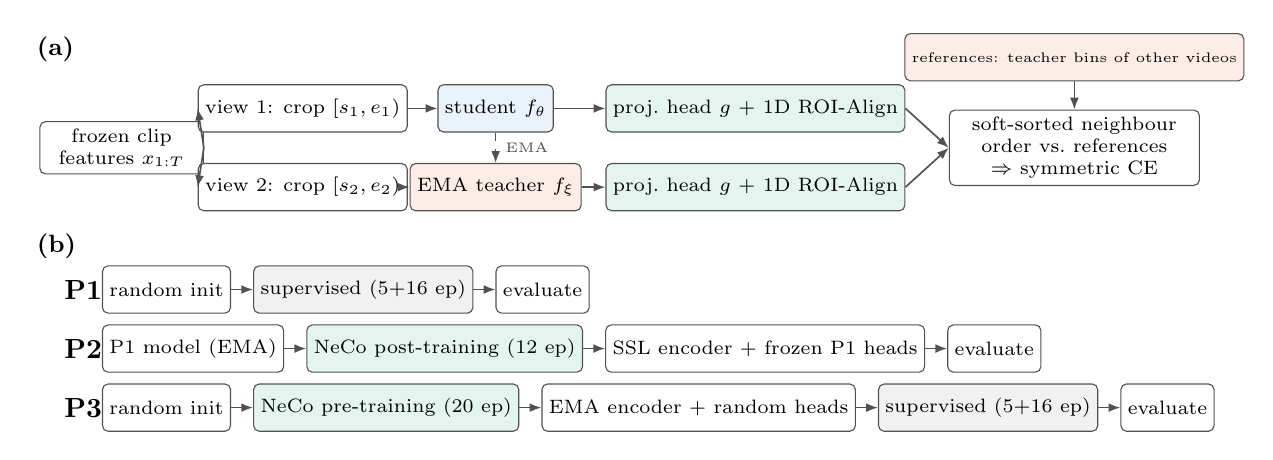
\begin{tikzpicture}[font=\scriptsize,
  box/.style={draw=cgray, rounded corners=2pt, align=center, inner sep=2.5pt, minimum height=0.6cm, fill=white},
  sbox/.style={box, fill=cblue!10}, tbox/.style={box, fill=corange!12}, hbox/.style={box, fill=caqua!12},
  arr/.style={-{Latex[length=1.5mm]}, semithick, cgray}]
% ---------------- (a) objective
\node[font=\small\bfseries, anchor=west] at (-0.2, 0.75) {(a)};
\node[box, text width=1.9cm] (x) at (1.0,-0.5) {frozen clip features $x_{1:T}$};
\node[box] (v1) at (3.3, 0.0) {view 1: crop $[s_1,e_1)$};
\node[box] (v2) at (3.3,-1.0) {view 2: crop $[s_2,e_2)$};
\node[sbox] (s) at (5.75, 0.0) {student $f_\theta$};
\node[tbox] (t) at (5.75,-1.0) {EMA teacher $f_\xi$};
\node[hbox] (g1) at (9.05, 0.0) {proj.\ head $g$ + 1D ROI-Align};
\node[hbox] (g2) at (9.05,-1.0) {proj.\ head $g$ + 1D ROI-Align};
\node[box, text width=3.0cm] (L) at (13.1,-0.5) {soft-sorted neighbour\\order vs.\ references\\$\Rightarrow$ symmetric CE};
\node[box, font=\tiny, fill=corange!12] (R) at (13.1, 0.65) {references: teacher bins of other videos};
\draw[arr] (x.east) -- (v1.west); \draw[arr] (x.east) -- (v2.west);
\draw[arr] (v1) -- (s); \draw[arr] (v2) -- (t);
\draw[arr] (s) -- (g1); \draw[arr] (t) -- (g2);
\draw[arr] (g1.east) -- (L.west); \draw[arr] (g2.east) -- (L.west); \draw[arr] (R) -- (L);
\draw[arr, dashed] (s) -- node[right, font=\tiny]{EMA} (t);
% ---------------- (b) protocols
\node[font=\small\bfseries, anchor=west] at (-0.2,-1.75) {(b)};
\def\gap{0.28cm}
\node[font=\bfseries, anchor=west] at (0.15,-2.3) {P1};
\node[box, anchor=west] (p1a) at (0.75,-2.3) {random init};
\node[box, right=\gap of p1a, fill=cgray!8] (p1b) {supervised (5+16 ep)};
\node[box, right=\gap of p1b] (p1c) {evaluate};
\draw[arr] (p1a) -- (p1b); \draw[arr] (p1b) -- (p1c);
\node[font=\bfseries, anchor=west] at (0.15,-3.05) {P2};
\node[box, anchor=west] (p2a) at (0.75,-3.05) {P1 model (EMA)};
\node[box, right=\gap of p2a, fill=caqua!12] (p2b) {NeCo post-training (12 ep)};
\node[box, right=\gap of p2b] (p2c) {SSL encoder + frozen P1 heads};
\node[box, right=\gap of p2c] (p2d) {evaluate};
\draw[arr] (p2a) -- (p2b); \draw[arr] (p2b) -- (p2c); \draw[arr] (p2c) -- (p2d);
\node[font=\bfseries, anchor=west] at (0.15,-3.8) {P3};
\node[box, anchor=west] (p3a) at (0.75,-3.8) {random init};
\node[box, right=\gap of p3a, fill=caqua!12] (p3b) {NeCo pre-training (20 ep)};
\node[box, right=\gap of p3b] (p3c) {EMA encoder + random heads};
\node[box, right=\gap of p3c, fill=cgray!8] (p3d) {supervised (5+16 ep)};
\node[box, right=\gap of p3d] (p3e) {evaluate};
\draw[arr] (p3a) -- (p3b); \draw[arr] (p3b) -- (p3c); \draw[arr] (p3c) -- (p3d); \draw[arr] (p3d) -- (p3e);
\end{tikzpicture}
\end{document}
